\section{Experimental Results and Evaluation} \label{section:benchmark}

This section describes the design of five benchmarks ($F_{1-10}$, $FA_{1-6}$, $CLS_{1-7}$, $CLU_{1}$, $IGC_{1}$), presents the results of the measurements and discusses their significance.

%\section{Benchmark} \label{section:benchmark}

%This section describes all benchmark components and how they will be evaluated. The benchmark consists of a mathematical function optimization component and machine learning component.

\subsection{Mathematical Function Optimization ($F_{1-10}$)}

The functions $F_{1-10}$ for the mathematical function optimization benchmark have been taken from the 2005 CEC conference on continuous evolutionary optimization algorithms~\cite{suganthan2005problem}. Many functions from the well known DeJong test-bed are included~\cite{Whitley1996245}.

For all functions $x=[x_1,x_2,x_3,...,x_D]$ are the input parameters, $o=[o_1,o_2,o_3,...,o_D]$ is the global optimum, $D$ is the dimension and $M$ is an orthogonal matrix with parameters unique to each function. The matrices for $o$ and $M$ can be obtained from~\cite{suganthan2005problem}.
The functions are illustrated in two dimensions in figures~\ref{f1},~\ref{f2},~\ref{f3},~\ref{f4},~\ref{f5},~\ref{f6},~\ref{f7},~\ref{f8},~\ref{f9} and~\ref{f10}. The benchmark parameters and settings are listed in table~\ref{table:f1-10_params}.

\begin{table}[H]
  \centering
  \begin{center}
    \footnotesize
    \begin{tabular}{ | c | c | c | c | }
      \hline
      Parameter & Value (D=10) & Value (D=30) & Value (D=50) \\ \hline
      Repeat measurements & 30 & 30 & 30 \\ \hline
      Generations & 667 & 1200 & 1429 \\ \hline
      Population Size & 150 & 250 & 350 \\ \hline
    \end{tabular}
  \end{center}
  \caption{Benchmark parameters for $F_{1-10}$}
  \label{table:f1-10_params}
\end{table}

\paragraph{Shifted Sphere Function ($F_1$)} Unimodal, Separable

\begin{minipage}{.5\textwidth}
  \[
    F_1(x)=\sum_{i=1}^{D}{z_i^2}
  \]
  \[ z=x-o \]
  \[ x \in [-100,100]^D \]
\end{minipage}%
\begin{minipage}{.5\textwidth}
  \begin{figure}[H]
    \centering
    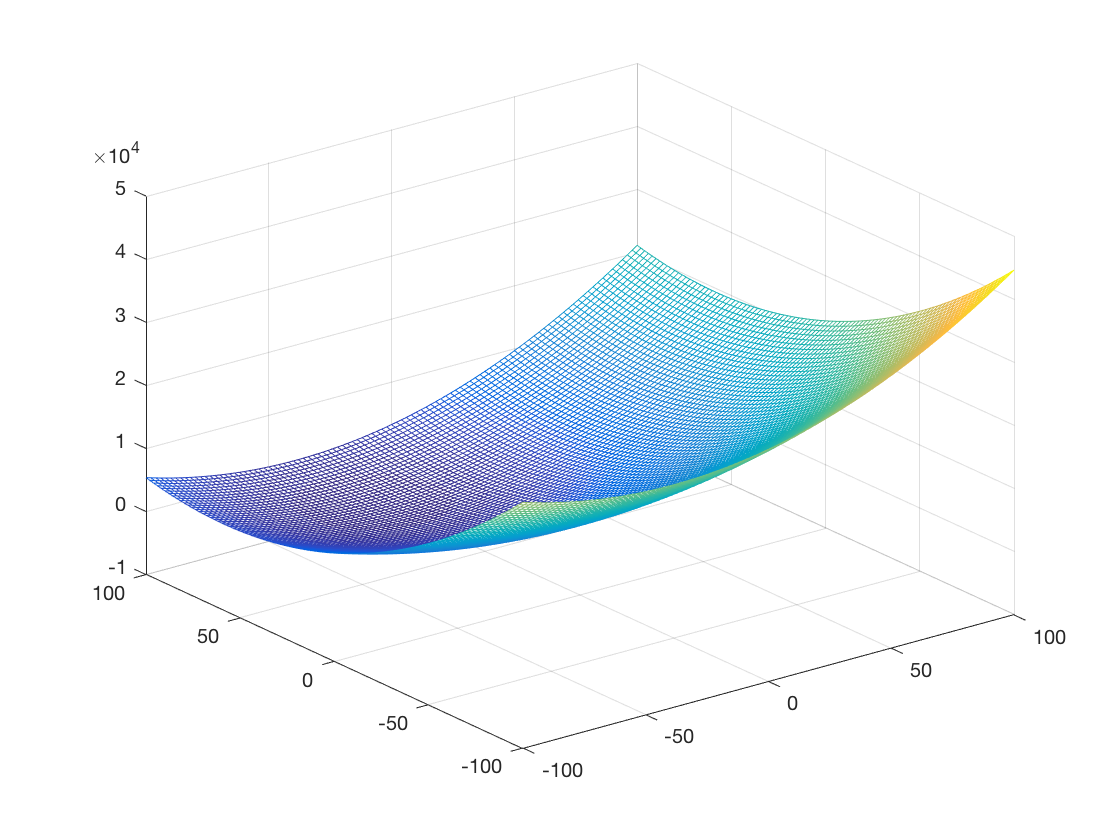
\includegraphics[width=0.7\linewidth]{f1}
    \caption{3-D map for 2-D function}
    \label{f1}
  \end{figure}
\end{minipage}


\paragraph{Shifted Schwefel’s Problem ($F_2$)} Unimodal, Non-Separable

\begin{minipage}{.5\textwidth}
\[
  F_2(x)=\sum_{i=1}^{D}{(\sum_{j=1}^{i}{z_j})^2}
\]
\[ z=x-o \]
\[ x \in [-100,100]^D \]
\end{minipage}%
\begin{minipage}{.5\textwidth}
  \begin{figure}[H]
    \centering
    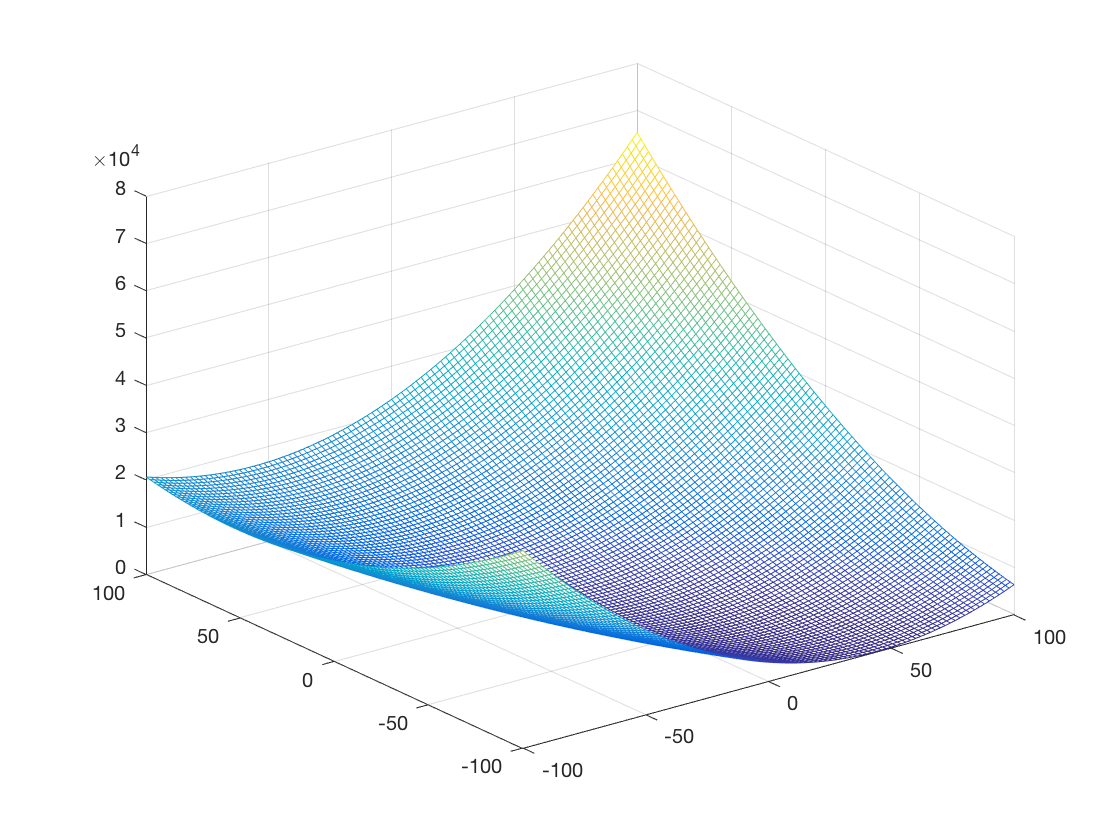
\includegraphics[width=0.7\linewidth]{f2}
    \caption{3-D map for 2-D function}
    \label{f2}
  \end{figure}
\end{minipage}


\paragraph{Shifted Rotated High Conditioned Elliptic Function ($F_3$)} Unimodal, Non-Separable

\begin{minipage}{.5\textwidth}
\[
  F_3(x)=\sum_{i=1}^{D}{(10^6)^{\frac{i-1}{D-1}}z_i^2}
\]
\[ z=(x-o)*M \]
\[ x \in [-100,100]^D \]
\end{minipage}%
\begin{minipage}{.5\textwidth}
  \begin{figure}[H]
    \centering
    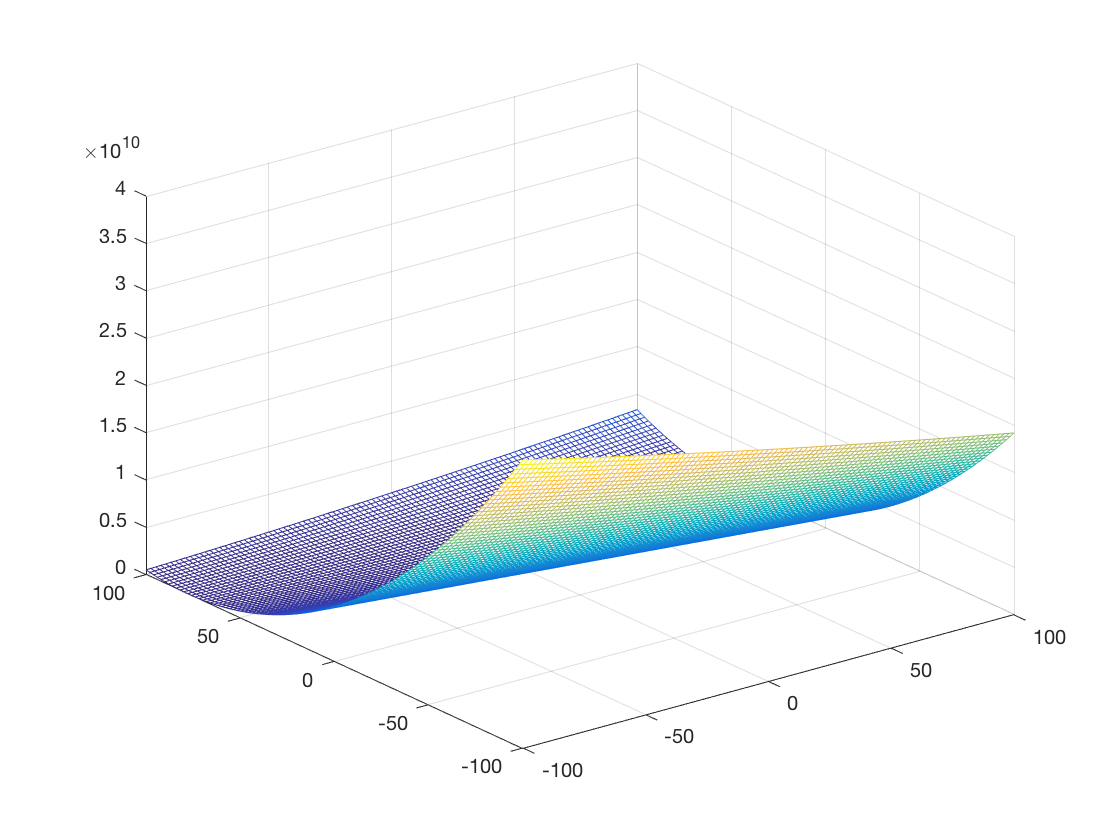
\includegraphics[width=0.7\linewidth]{f3}
    \caption{3-D map for 2-D function}
    \label{f3}
  \end{figure}
\end{minipage}


\paragraph{Shifted Schwefel’s Problem with Noise in Fitness ($F_4$)} Unimodal, Non-Separable

\begin{minipage}{.5\textwidth}
\[
  F_4(x)=(\sum_{i=1}^{D}{(\sum_{j=1}^{i}{z_j})^2})*(1+0.4|N(0,1)|)
\]
\[ z=x-o \]
\[ x \in [-100,100]^D \]
\end{minipage}%
\begin{minipage}{.5\textwidth}
  \begin{figure}[H]
    \centering
    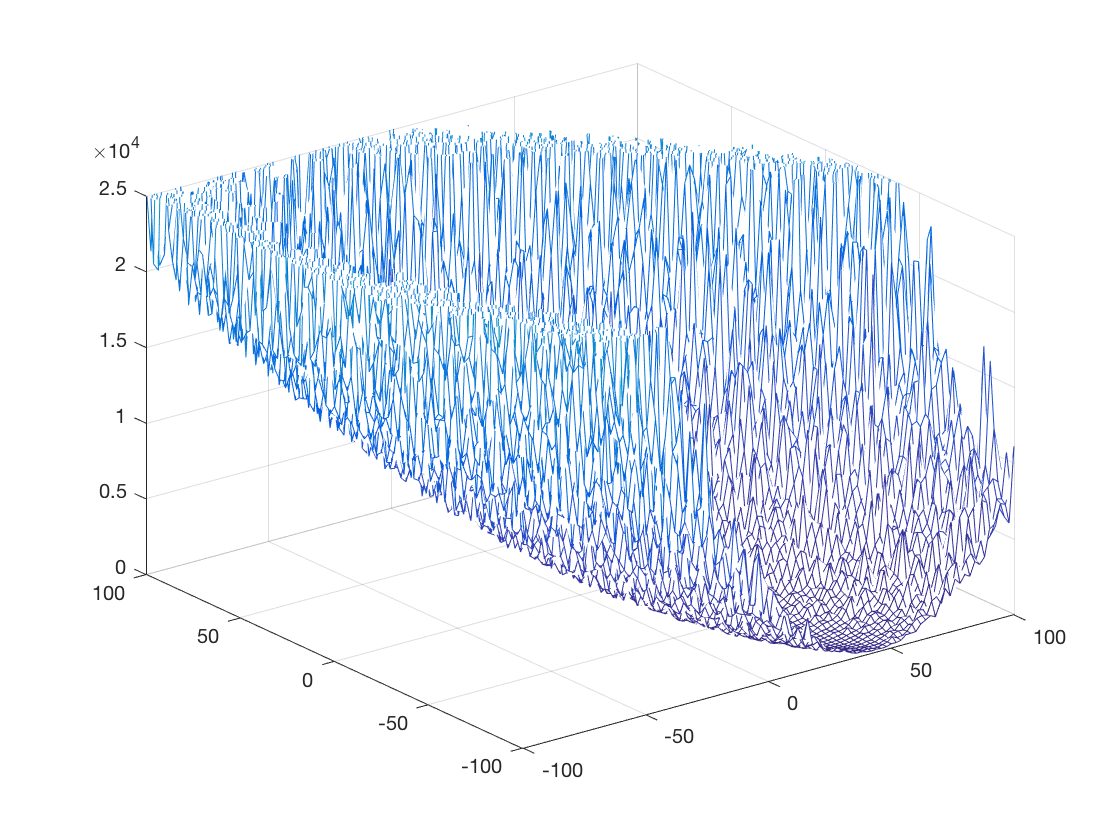
\includegraphics[width=0.7\linewidth]{f4}
    \caption{3-D map for 2-D function}
    \label{f4}
  \end{figure}
\end{minipage}


\paragraph{Schwefel’s Problem with Global Optimum on Bounds ($F_5$)} Unimodal, Non-Separable

\begin{minipage}{.5\textwidth}
\[
  F_5(x)=max\{|A_ix-B_i|\}
\]
\[ i=1,...,D, x \in [-100,100]^D \]
\[ A \text{ is a } D*D \text{ matrix}, a_{ij} = \text{ random numbers in } [-500,500],  det(A) \neq 0 \]
\[ B_i = A_i * o, o_i = \text{ random numbers in } [-100,100] \]
\[ o_i = -100 \text{, for } i=1,2,...,[D/4], o_i = 100 \text{, for } i=[3D/4],...,D \]
\end{minipage}%
\begin{minipage}{.5\textwidth}
  \begin{figure}[H]
    \centering
    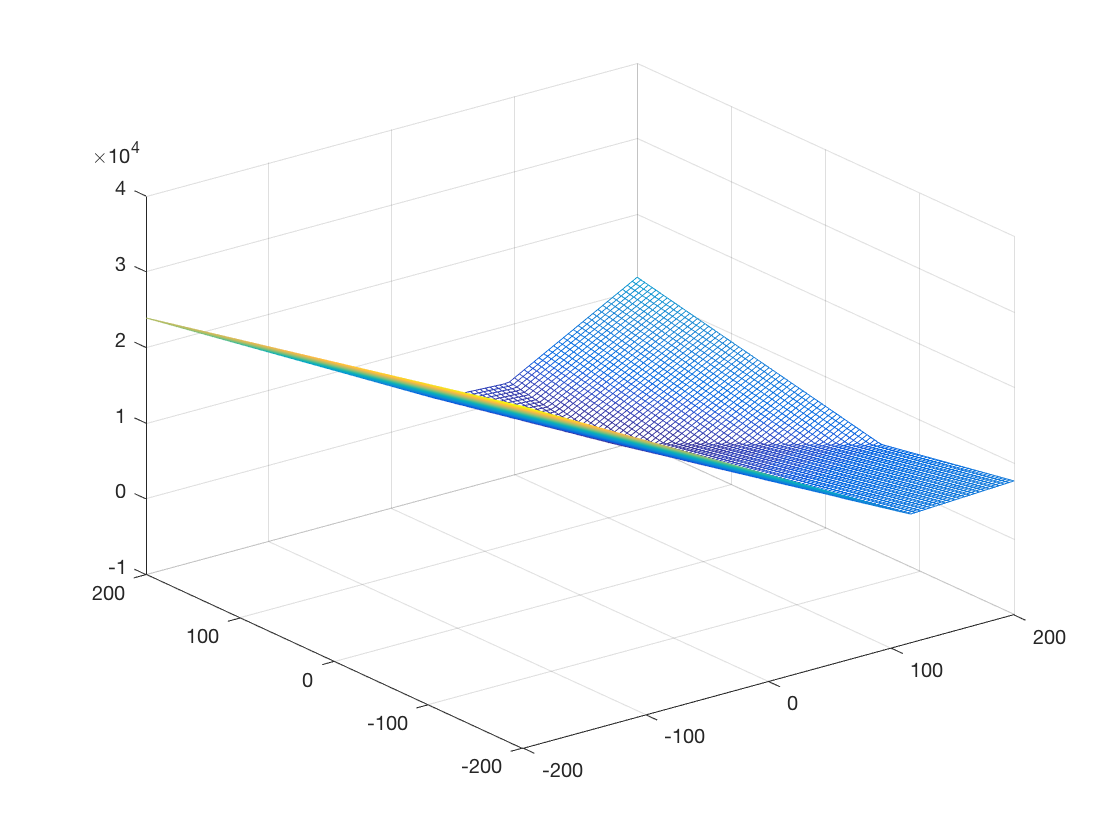
\includegraphics[width=0.7\linewidth]{f5}
    \caption{3-D map for 2-D function}
    \label{f5}
  \end{figure}
\end{minipage}


\paragraph{Shifted Rosenbrock’s Function ($F_6$)} Multimodal, Non-Separable

\begin{minipage}{.5\textwidth}
\[
  F_6(x)=\sum_{i=1}^{D-1}{(100(z_i^2 - z_{i+1})^2 + (z_i - 1)^2)}
\]
\[ z=x-o+1 \]
\[ x \in [-100,100]^D \]
\end{minipage}%
\begin{minipage}{.5\textwidth}
  \begin{figure}[H]
    \centering
    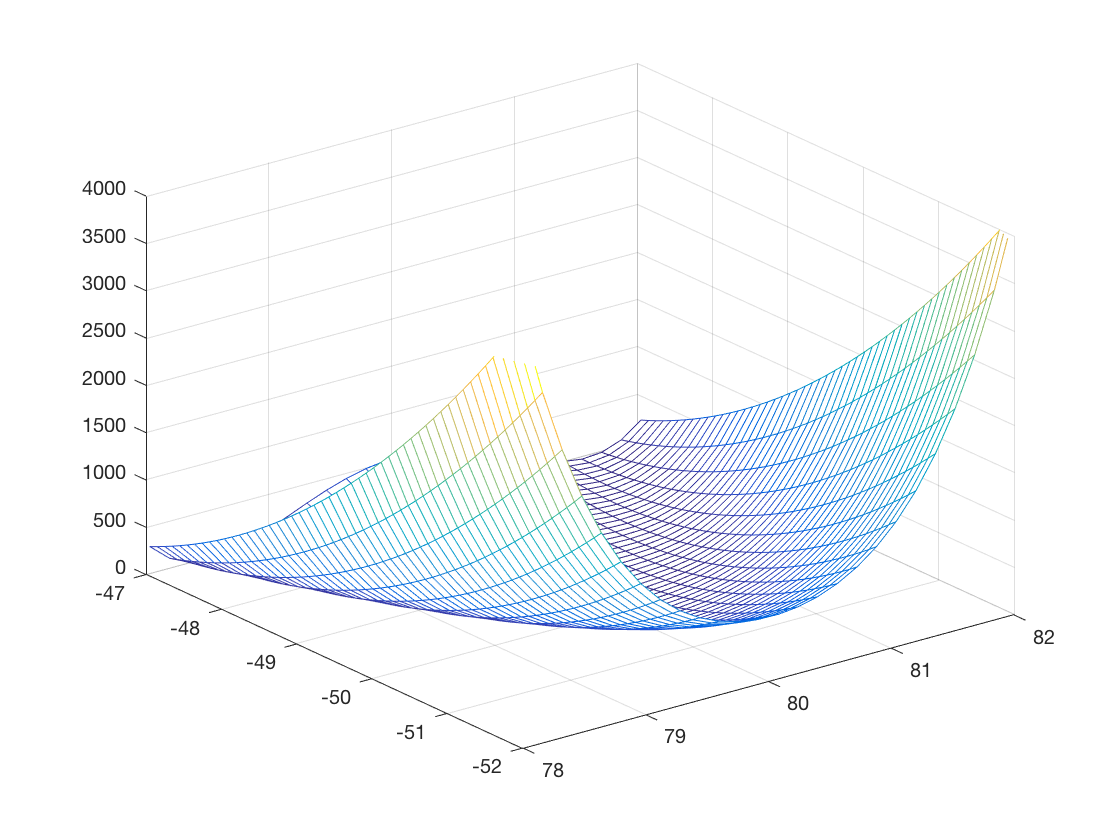
\includegraphics[width=0.7\linewidth]{f6}
    \caption{3-D map for 2-D function}
    \label{f6}
  \end{figure}
\end{minipage}


\paragraph{Shifted Rotated Griewank’s Function without Bounds ($F_7$)} Multimodal, Non-Separable

\begin{minipage}{.5\textwidth}
\[
  F_7(x)=\sum_{i=1}^{D}{\frac{z_i^2}{4000}}-\prod_{i=1}^{D}{\cos{\frac{z_i}{\sqrt{i}}}}+1
\]
\[ z=(x-o)*M \]
\[ x \in [0,600]^D \]
\end{minipage}%
\begin{minipage}{.5\textwidth}
  \begin{figure}[H]
    \centering
    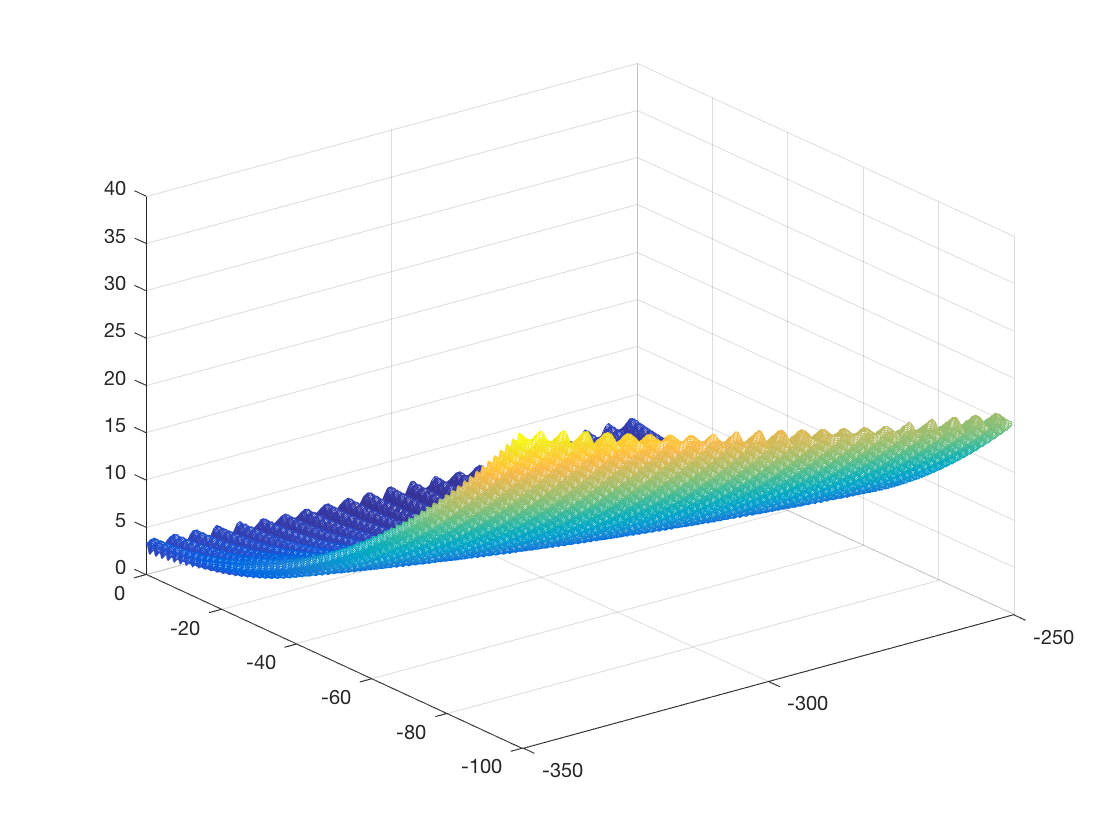
\includegraphics[width=0.7\linewidth]{f7}
    \caption{3-D map for 2-D function}
    \label{f7}
  \end{figure}
\end{minipage}

\paragraph{Shifted Rotated Ackley’s Function with Global Optimum on Bounds ($F_8$)} Multimodal, Non-Separable

\begin{minipage}{.5\textwidth}
\[
  F_8(x)=-20\exp{(-0.2\sqrt{\frac{1}{D}\sum_{i=1}^{D}{z_i^2}})}-\exp{(\frac{1}{D}\sum_{i=1}^{D}{\cos{(2\pi z_i)}})} + 20 + e
\]
\[ z=(x-o)*M \]
\[ x \in [-32,32]^D \]
\end{minipage}%
\begin{minipage}{.5\textwidth}
  \begin{figure}[H]
    \centering
    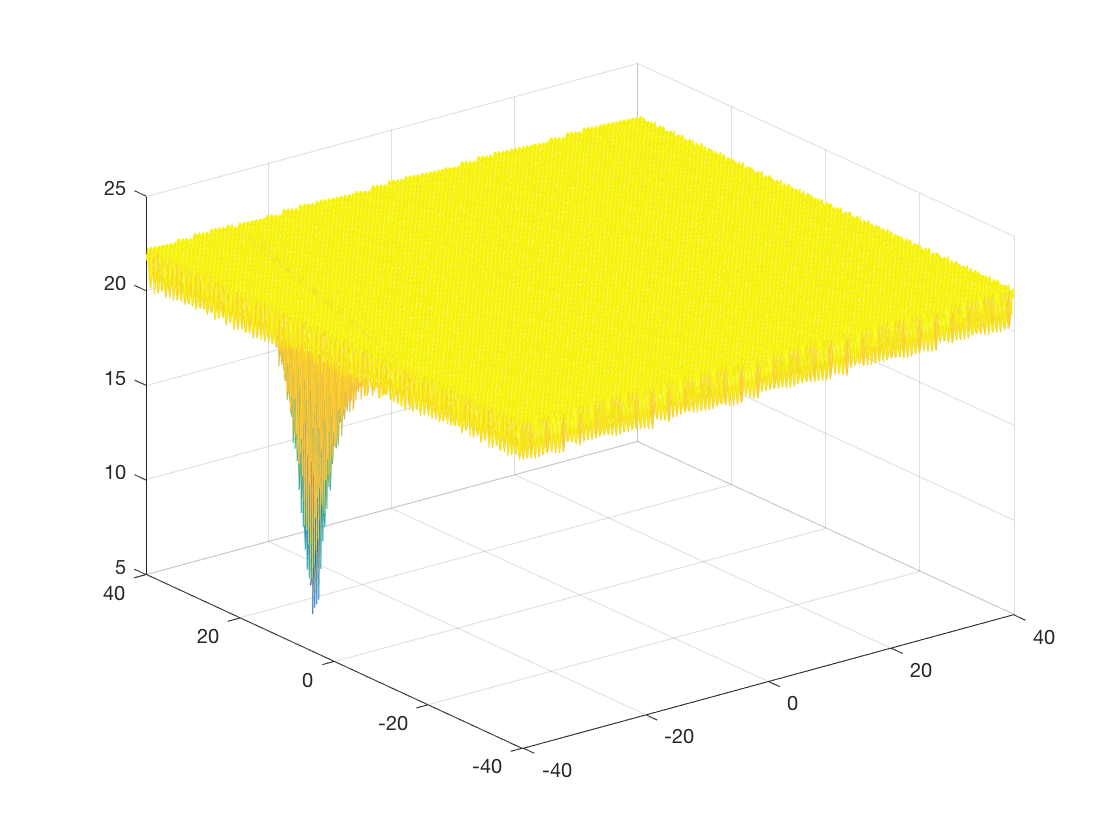
\includegraphics[width=0.7\linewidth]{f8}
    \caption{3-D map for 2-D function}
    \label{f8}
  \end{figure}
\end{minipage}

\paragraph{Shifted Rastrigin’s Function ($F_9$)} Multimodal, Separable

\begin{minipage}{.5\textwidth}
\[
  F_9(x)=\sum_{i=1}^{D}{z_i^2 - 10\cos{(2\pi z_i)} + 10}
\]
\[ z=x-o \]
\[ x \in [-5,5]^D \]
\end{minipage}%
\begin{minipage}{.5\textwidth}
  \begin{figure}[H]
    \centering
    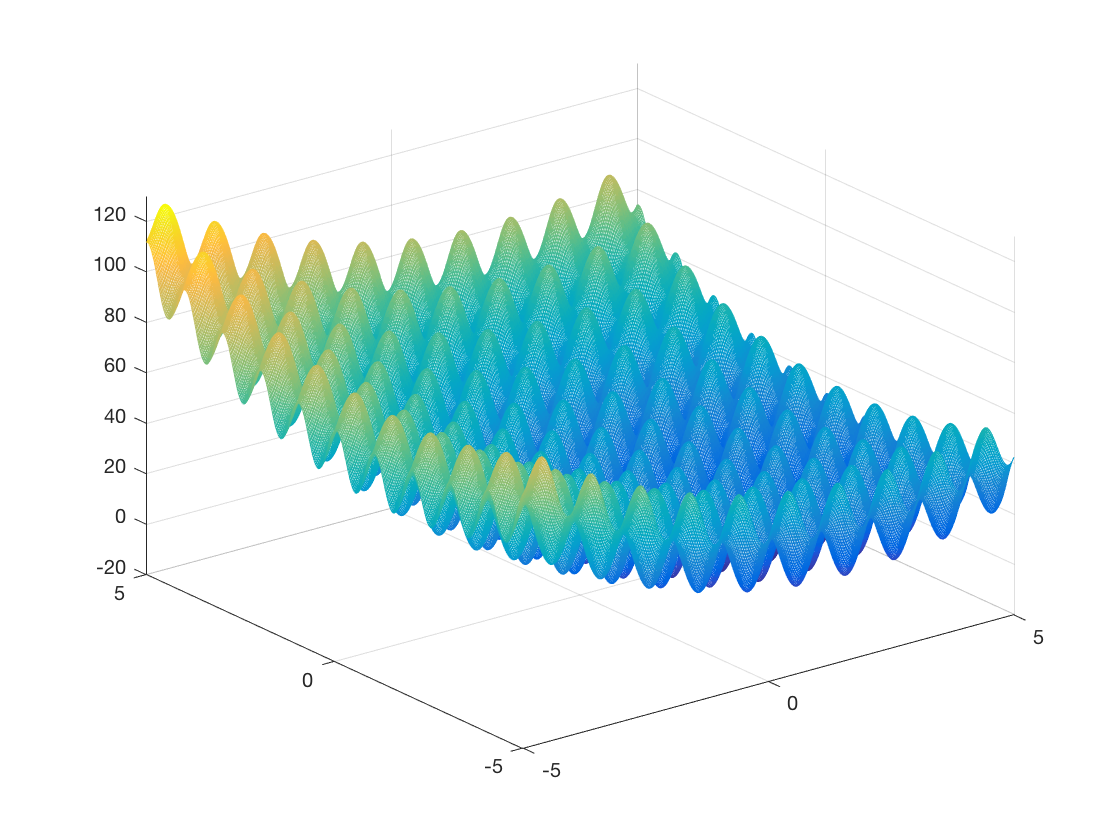
\includegraphics[width=0.7\linewidth]{f9}
    \caption{3-D map for 2-D function}
    \label{f9}
  \end{figure}
\end{minipage}


\paragraph{Shifted Rotated Rastrigin’s Function ($F_{10}$)} Multimodal, Non-Separable

\begin{minipage}{.5\textwidth}
\[
  F_{10}(x)=\sum_{i=1}^{D}{z_i^2 - 10\cos{(2\pi z_i)} + 10}
\]
\[ z=(x-o)*M \]
\[ x \in [-5,5]^D \]
\end{minipage}%
\begin{minipage}{.5\textwidth}
  \begin{figure}[H]
    \centering
    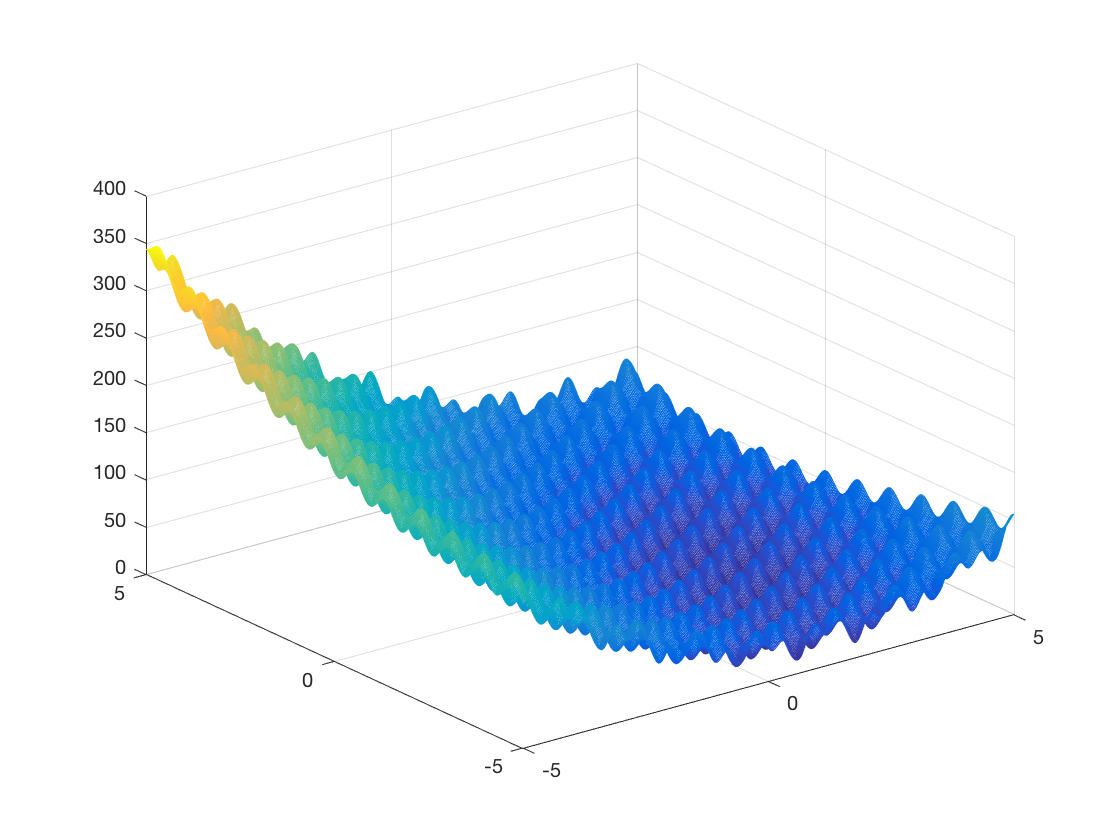
\includegraphics[width=0.7\linewidth]{f10}
    \caption{3-D map for 2-D function}
    \label{f10}
  \end{figure}
\end{minipage}

%\subsection{Machine Learning}

%This section describes the machine learning benchmarks, which primarily utilize feed-forward neural networks.

%To evaluate the optimization algorithms further I set have set out to apply them on a variety of machine learning problems. These will predominantly be applications of feed-forward neural networks (FFNN). The design of the neural network is one input layer with a size based on the problem dimension, two hidden layers and one output layer. I have chosen to use two hidden layers to make sure a good solution can be found quickly~\cite{329294}. The size of the hidden layers was set to $2/3$ and $1/3$ of the mean of the size of the input and output layers.

\subsection{Function Approximation ($FA_{1-6}$)}

The optimization algorithms were used find the optimal weights for feed-forward neural networks. The neural networks were evaluated on six function approximation data-sets which are available in Matlab's Neural Network Toolbox. The benchmark parameters and settings are listed in table~\ref{table:fa1-6_params}. The data-sets are listed in table~\ref{table:fa1-6_data-sets}.

\begin{table}[H]
  \centering
  \begin{center}
    \footnotesize
    \begin{tabular}{ | c | c | }
      \hline
      Parameter & Value \\ \hline
      Repeat measurements & 5 \\ \hline
      Generations & 250 \\ \hline
      Population Size & 50 \\ \hline
    \end{tabular}
  \end{center}
  \caption{Benchmark parameters for $FA_{1-6}$}
  \label{table:fa1-6_params}
\end{table}

\begin{table}[H]
  \centering
  \begin{center}
    \footnotesize
    \begin{tabular}{ | c | c | c | c | c | }
      \hline
      Data-set & Description & Input-Dimension & Output-Dimension & Weight-Dimension \\ \hline
      simplefit & Simple fitting & 1 & 1 & 4 \\ \hline
      bodyfat & Body fat percentage & 13 & 1 & 196 \\ \hline
      chemical & Chemical sensor & 8 & 1 & 81 \\ \hline
      cho & Cholesterol & 21 & 3 & 528 \\ \hline
      engine & Engine behavior  & 2 & 2 & 12 \\ \hline
      house & House value & 13 & 1 & 196 \\ \hline
    \end{tabular}
  \end{center}
  \caption{Data-sets for $FA_{1-6}$}
  \label{table:fa1-6_data-sets}
\end{table}

\paragraph{Evalutation Procedure}

The data sets contain two matrices. One with sample input vectors to the neural network and one with the expected correct output vectors. The function which the optimization algorithm directly optimizes is the sum of squared errors as defined by equation~\ref{eq:fa_fitness}

\begin{equation} \label{eq:fa_fitness}
  sse(x,t) = \frac{1}{2n} \sum_{i=1}^{n}{(y(x)-t)^2}
\end{equation}

where $x$ is the input vector to neural network $y$, $t$ is the correct expected output which $y(x)$ should produce and n is the length of vector $x$.

\subsection{Classification ($CLS_{1-7}$)}

The optimization algorithms were used find the optimal weights for feed-forward neural networks. The neural networks were evaluated on seven classification data-sets which are available in Matlab's Neural Network Toolbox. The benchmark parameters and settings are listed in table~\ref{table:cls1-7_params}. The data-sets are listed in table~\ref{table:cls1-7_data-sets}.

\begin{table}[H]
  \centering
  \begin{center}
    \footnotesize
    \begin{tabular}{ | c | c | }
      \hline
      Parameter & Value \\ \hline
      Repeat measurements & 5 \\ \hline
      Generations & 250 \\ \hline
      Population Size & 50 \\ \hline
    \end{tabular}
  \end{center}
  \caption{Benchmark parameters for $CLS_{1-7}$}
  \label{table:cls1-7_params}
\end{table}

\begin{table}[H]
  \centering
  \begin{center}
    \footnotesize
    \begin{tabular}{ | c | c | c | c | c | }
      \hline
      Data-set & Description & Input-Dimension & Output-Dimension & Weight-Dimension \\ \hline
      simpleclass & imple pattern recognition & 2 & 4 & 18 \\ \hline
      cancer & Breast cancer & 9 & 2 & 110 \\ \hline
      crab & Crab gender & 6 & 2 & 56 \\ \hline
      glass & Glass chemical & 9 & 2 & 110 \\ \hline
      iris & Iris flower & 4 & 3 & 35 \\ \hline
      thyroid & Thyroid function  & 21 & 3 & 528 \\ \hline
      wine & Italian wines & 13 & 3 & 224 \\ \hline
    \end{tabular}
  \end{center}
  \caption{Data-sets for $CLS_{1-7}$}
  \label{table:cls1-7_data-sets}
\end{table}


\paragraph{Evalutation Procedure}

Same as $FA_{1-6}$.

\subsection{Clustering ($CLU_{1}$)}

The optimization algorithms were used find the optimal weights for feed-forward neural networks. The neural networks were evaluated on one clustering data-set which is available in Matlab's Neural Network Toolbox. The benchmark parameters and settings are listed in table~\ref{table:clu1_params}. The data-sets are listed in table~\ref{table:clu1_data-sets}.

\begin{table}[H]
  \centering
  \begin{center}
    \footnotesize
    \begin{tabular}{ | c | c | }
      \hline
      Parameter & Value \\ \hline
      Repeat measurements & 5 \\ \hline
      Generations & 250 \\ \hline
      Population Size & 50 \\ \hline
    \end{tabular}
  \end{center}
  \caption{Benchmark parameters for $CLU_{1}$}
  \label{table:clu1_params}
\end{table}

\begin{table}[H]
  \centering
  \begin{center}
    \footnotesize
    \begin{tabular}{ | c | c | c | c | c | }
      \hline
      Data-set & Description & Input-Dimension & Output-Dimension & Weight-Dimension \\ \hline
      simplecluster & Simple clustering & 2 & 4 & 18 \\ \hline
    \end{tabular}
  \end{center}
  \caption{Data-sets for $CLU_{1}$}
  \label{table:clu1_data-sets}
\end{table}


\paragraph{Evalutation Procedure}

Same as $FA_{1-6}$.

\subsection{Intelligent Game Controllers ($IGC_{1}$)}


Machine learning test set $IGC_{1}$ uses evolutionary algorithms to evolve weights for feed-forward neural networks, which control the behavior of a game-agent in the classic game of ``Snake''. The benchmark parameters and settings are listed in table~\ref{table:fa1-6_params}.

\begin{table}[H]
  \centering
  \begin{center}
    \footnotesize
    \begin{tabular}{ | c | c | c | c | }
      \hline
      Parameter & Value  \\ \hline
      Individuals & 140 \\ \hline
      Generations & 1000 \\ \hline
      Grid dimension & 10*10 \\ \hline
      Weight dimension & 140 \\ \hline
      Repeat measurements & 10 \\ \hline
      Repeat fitness measurements & 5 \\ \hline
    \end{tabular}
  \end{center}
  \caption{Benchmark parameters for $FA_{1-6}$}
  \label{table:fa1-6_params}
\end{table}

\paragraph{Game Description and Rules}

The game is made up of a $n*m$ square grid through which a snake can freely move. The snake consists of a sequence of interconnected blocks and is divided into a head which moves in a certain direction and a tail which follows the head. Food blocks randomly appear on block at a time on the grid and the snake's objective is eat these blocks. When the snake's head touches the food block the block vanishes and the snake grows one square in length. If the head of the snake tries to move outside the grid it dies and the game ends. If the head of the snake collides with the tail it also and dies and the game ends. The snake's head can move in four direction: up, down, left and right. If the snake tries to move in the opposite of it's current direction it also dies. The snake has a starvation counter which forces it to pursue food and eat. The starvation counter is initialized to the starvation threshold when the game begins and decreases by one every time the snake moves. When the snake eats, the starvation counter is increased once by the starvation threshold. Figure~\ref{snake} illustrates the game grid. Figure~\ref{snake_alg} described the algorithm for the game. The game's parameters are explained in table~\ref{snake_p}.

\begin{figure}[H]
  \centering
  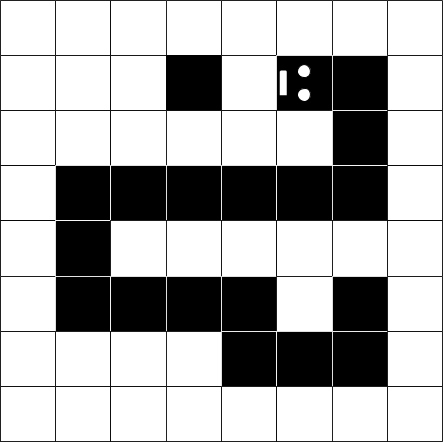
\includegraphics[width=.3\linewidth]{snake}
  \caption{Snake $8*8$ game-field with snake hunting food}
  \label{snake}
\end{figure}


\begin{table}[H]
  \centering
  \begin{center}
    \begin{tabular}{ | c | c | }
      \hline
      Parameter & Description \\ \hline
      $D^2$ & Dimension of grid ($m*n$ blocks) \\ \hline
      $(x,y)$ & Starting point for snake head \\ \hline
      $d_s$ & Starting direction for snake head ($=\{left,right,up,down\}$) \\ \hline
      $t$ & Starvation threshold \\ \hline
    \end{tabular}
  \end{center}
  \caption{Parameters snake game}
  \label{snake_p}
\end{table}


\paragraph{Representation of Game State}

In order to control the snake with a neural network a representation of the state of the game has to be generated before each move. The chosen representation is a 12-dimensional vector in the range $[0,1]$. The initial default value of all dimensions is zero. Dimensions 1-4 indicates with a value of one whether any dangerous object (the tail or the edge of the grid) is immediately to the left, to the right, above or below the snake's head. Dimensions 5-8 indicate the distribution of the tail relative to the head of the snake. Floating-point numbers indicate how much of the tail is above, below, to the right and to the left of the head. Dimensions 9-12 indicate with a value of one when food is to the left, to the right, above or below the snake's head.

\begin{algorithm}[h]

  \caption{Snake game}
  \label{snake_alg}
    \begin{algorithmic}
      \State $initializeSnake()$
      \State $foodEaten \gets 0$
      \State $movesMade \gets 0$
      \While{$alive$}
        \State $state \gets getGameState()$
        \State $move \gets getNextMove(state)$
        \State $moveSnake(move)$
        \If{$collides(head,tail)$} $die()$
        \EndIf
        \If{$outOfBounds(head)$} $die$
        \EndIf
        \If{$collides(head,food)$}
          \State{$eatFood(food)$}
          \State{$growSnake()$}
          \State{$foodEaten \gets foodEaten + 1$}
        \EndIf
        \State{$movesMade \gets movesMade + 1$}
      \EndWhile
      \State{\Return $foodEaten + sigmoid(movesMade)$}

    \end{algorithmic}
\end{algorithm}

\paragraph{Neural Network Controller}

The neural network which controls is a feed-forward neural network with one hidden layer. The input layer has 12 neurons which correspond to the game-state representation. The output layer has four neurons, which correspond to the decision to move left, right, up or down. The hidden layer has 8 neurons. Figure \ref{ffnn_snake} illustrates the network.





\begin{figure}[H]
  \centering

  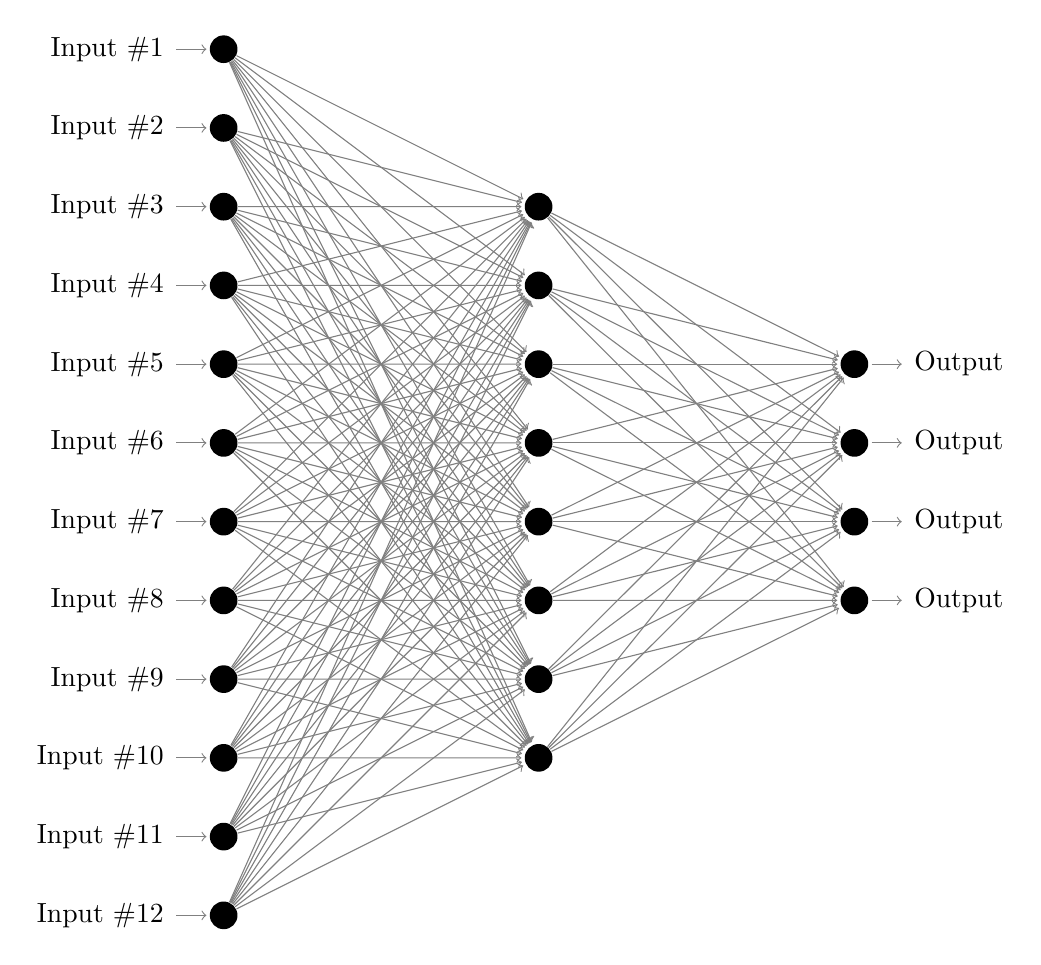
\begin{tikzpicture}[shorten >=1pt,->,draw=black!50, node distance=.3\layersep]
      \tikzstyle{every pin edge}=[<-,shorten <=1pt]
      \tikzstyle{neuron}=[circle,fill=black,minimum size=10pt,inner sep=0pt]
      \tikzstyle{input neuron}=[neuron];
      \tikzstyle{output neuron}=[neuron];
      \tikzstyle{hidden neuron}=[neuron];
      \tikzstyle{annot} = [text width=2em, text centered]

      % Draw the input layer nodes
      \foreach \name / \y in {1,...,12}
      % This is the same as writing \foreach \name / \y in {1/1,2/2,3/3,4/4}
          \node[input neuron, pin=left:Input \#\y] (I-\name) at (0,-\y) {};

      % Draw the hidden layer nodes
      \foreach \name / \y in {1,...,8}
          \path[yshift=-2cm]
              node[hidden neuron] (H-\name) at (4\layersep,-\y cm) {};

      % Draw the hidden layer nodes
      \foreach \name / \y in {1,...,4}
          \path[yshift=-4cm]
              node[output neuron, pin={[pin edge={->}]right:Output}, right of=H-3] (O-\name) at (8\layersep,-\y cm) {};


      % Connect every node in the input layer with every node in the
      % hidden layer.
      \foreach \source in {1,...,12}
          \foreach \dest in {1,...,8}
              \path (I-\source) edge (H-\dest);

      % Connect every node in the hidden layer with the output layer
      \foreach \source in {1,...,8}
          \foreach \dest in {1,...,4}
              \path (H-\source) edge (O-\dest);
  \end{tikzpicture}

  \caption{FFNN snake controller}
  \label{ffnn_snake}
\end{figure}

\paragraph{Fitness Function and Evaluation}

The objective function, which is run by the optimization algorithms, takes the evolved weights of the neural network and attempts to play the game using them. The fitness function of gameplay if determined by the equation~\ref{eq:snake_fitness}.

\begin{equation} \label{eq:snake_fitness}
  fitness = \text{foodEaten} + \frac{1}{1-e^{-\text{movesMade}}}
\end{equation}

The fitness function ensured that the snake has an ``easy start'' when it will be rewarded for not dying, but then has to pursue food in order to maximize it's fitness.


\subsection{Results}

This section presents results for the benchmarks of the four algorithms presented in this thesis.

\paragraph{Function Optimization at D=10}
DEDA significantly outperforms the other algorithms at most unimodal functions. DE significantly outperforms the others at one unimodal and one multimodal function. PSO outperforms the others by a slight margin on most multimodal function. Separability does not seem to influence the results. Table~\ref{table:f_res_10} presents the data.

For $F_1$ EDA significantly outperforms DE and PSO, while DEDA lags far behind. For $F_2$ DEDA finds significantly better results than the rest, while EDA performs the worst. For $F_3$ DEDA performs best followed by DE, but PSO and EDA do not find good solutions at all. For $F_4$ DEDA significantly outperforms the rest and EDA does not find any good results at all. For $F_5$ DE significantly outperforms the rest, DEDA finds an acceptable results and PSO and EDA do not find any good results. For $F_6$ DE significantly outperforms the rest, DEDA finds an acceptable results and PSO and EDA do not find any good results. For $F_7$ EDA find the best solution but all algorithms achieve similar results. For $F_8$ PSO find the best solution but all algorithms achieve similar results. For $F_9$ PSO find the best solution but all algorithms achieve similar results. For $F_{10}$ PSO find the best solution but all algorithms achieve similar results.

\begin{table}[H]
  \centering
  \begin{center}
    \footnotesize
    \begin{tabular}{ | c | c | c | c | c | c | c | c | c | }
      \hline
      F & \multicolumn{2}{c|}{DE} & \multicolumn{2}{c|}{PSO} & \multicolumn{2}{c|}{EDA} & \multicolumn{2}{c |}{\textbf{DEDA}} \\ \hline
      & Avg & Std & Avg & Std & Avg & Std & Avg & Std \\ \hline
      1 & 3,88E-17 & 3,42E-17 & 1,65E-16 & 3,64E-16 & \textbf{1,67E-27} & 4,07E-28 & 0,00E+00 & 0,00E+00 \\ \hline
      2 & 1,83E-08 & 1,24E-08 & 2,07E-06 & 3,36E-06 & 2,51E+02 & 1,42E+02 & \textbf{4,23E-27} & 3,10E-27 \\ \hline
      3 & 5,19E-01 & 2,29E-01 & 4,88E+05 & 7,21E+05 & 1,09E+05 & 8,32E+04 & \textbf{4,96E-02} & 3,01E-02 \\ \hline
      4 & 3,36E-07 & 2,59E-07 & 6,31E-05 & 9,10E-05 & 3,21E+02 & 2,16E+02 & \textbf{1,73E-26} & 2,16E-26 \\ \hline
      5 & \textbf{4,24E-13} & 7,82E-13 & 4,94E+02 & 4,49E+02 & 1,67E+02 & 1,37E+02 & 6,57E+00 & 1,26E+01 \\ \hline
      6 & \textbf{5,43E-05} & 1,24E-04 & 2,11E+02 & 7,15E+02 & 1,34E+04 & 4,30E+04 & 6,71E+00 & 5,83E-01 \\ \hline
      7 & 4,87E-01 & 7,61E-02 & 2,74E-01 & 1,79E-01 & \textbf{1,87E-01} & 2,23E-01 & 3,41E-01 & 1,24E-01 \\ \hline
      8 & 2,04E+01 & 7,20E-02 & \textbf{2,03E+01} & 8,82E-02 & 2,04E+01 & 8,15E-02 & 2,04E+01 & 6,88E-02 \\ \hline
      9 & 2,50E+01 & 4,44E+00 & \textbf{1,76E+00} & 1,49E+00 & 2,35E+01 & 3,08E+00 & 1,80E+01 & 3,52E+00 \\ \hline
      10 & 3,26E+01 & 4,25E+00 & \textbf{1,73E+01} & 7,50E+00 & 2,11E+01 & 3,43E+00 & 2,05E+01 & 3,62E+00 \\ \hline
    \end{tabular}
  \end{center}
  \caption{Benchmark results for $F_{1-10}$ $D=10$}
  \label{table:f_res_10}
\end{table}

\paragraph{Function Optimization at D=30}
DEDA moderately outperform the other algorithms at most unimodal functions. PSO outperform all other algorithms on the multimodal functions, but the results are fairly even. DEDA significantly outperforms the others on separable unimodal algorithms. Table~\ref{table:f_res_30} presents the data.

For $F_1$ DEDA performs best closely followed by EDA. PSO also finds a good result but DE finds a significantly worse result. For $F_2$ all algorithms find similar solutions and DEDA finds the best one. For $F_3$ all algorithms find similar solutions and EDA finds the best one. For $F_4$ all algorithms find somewhat similar solutions and DEDA finds the best one. For $F_5$ all algorithms find somewhat similar solutions and DEDA finds the best one. For $F_6$ all algorithms find somewhat similar solutions and DEDA finds the best one. For $F_7$ PSO finds the best solution followed EDA and DE and  DEDA find worse solutions. For $F_8$ all algorithms find similar solutions and PSO finds the best one. For $F_9$ DE, EDA and DEDA find similar solutions, but PSO finds a somewhat better solution. For $F_{10}$ all algorithms find similar solutions and PSO finds the best one.

\begin{table}[H]
  \centering
  \begin{center}
    \footnotesize
    \begin{tabular}{ | c | c | c | c | c | c | c | c | c | }
      \hline
      F & \multicolumn{2}{c|}{DE} & \multicolumn{2}{c|}{PSO} & \multicolumn{2}{c|}{EDA} & \multicolumn{2}{c |}{\textbf{DEDA}} \\ \hline
      & Avg & Std & Avg & Std & Avg & Std & Avg & Std \\ \hline
      1 & 1,03E+00 & 1,53E-01 & 4,54E-10 & 7,66E-10 & 1,81E-25 & 7,66E-10 & \textbf{8,58E-28} & 1,40E-28 \\ \hline
      2 & 3,07E+03 & 6,91E+02 & 1,42E+03 & 7,01E+02 & 1,71E+03 & 7,01E+02 & \textbf{4,84E+02} & 1,80E+02 \\ \hline
      3 & 3,28E+07 & 5,84E+06 & 1,92E+07 & 1,12E+07 & \textbf{4,93E+06} & 1,12E+07 & 1,88E+07 & 4,86E+06 \\ \hline
      4 & 6,06E+03 & 1,23E+03 & 1,50E+04 & 6,87E+03 & 3,63E+03 & 6,87E+03 & \textbf{6,74E+02} & 1,96E+02 \\ \hline
      5 & 1,38E+03 & 3,54E+02 & 6,92E+03 & 2,55E+03 & 2,70E+03 & 2,55E+03 & \textbf{1,31E+02} & 9,21E+01 \\ \hline
      6 & 2,99E+03 & 1,24E+03 & \textbf{5,30E+02} & 8,60E+02 & 8,57E+04 & 8,60E+02 & 7,32E+03 & 2,21E+04 \\ \hline
      7 & 1,22E+00 & 5,36E-02 & \textbf{5,77E-02} & 5,18E-02 & 5,86E+00 & 5,18E-02 & 2,54E-01 & 4,25E-01 \\ \hline
      8 & 2,09E+01 & 4,24E-02 & \textbf{2,09E+01} & 5,74E-02 & 2,10E+01 & 5,74E-02 & 2,10E+01 & 5,41E-02 \\ \hline
      9 & 1,91E+02 & 9,58E+00 & \textbf{2,53E+01} & 5,97E+00 & 1,53E+02 & 5,97E+00 & 1,60E+02 & 8,27E+00 \\ \hline
      10 & 2,19E+02 & 1,09E+01 & \textbf{1,14E+02} & 3,78E+01 & 1,59E+02 & 3,78E+01 & 1,60E+02 & 8,53E+00 \\ \hline
    \end{tabular}
  \end{center}
  \caption{Benchmark results for $F_{1-10}$ $D=30$}
  \label{table:f_res_30}
\end{table}

\paragraph{Function Optimization at D=50}
The results are fairly even. DEDA significantly outperforms the others on separable unimodal algorithms. The multimodal functions favor PSO, the unimodal function favor UMDA while DEDA's results are more scattered. Table~\ref{table:f_res_50} presents the data.

For $F_1$ DEDA find the best results closely followed by EDA. DE finds a bad solution and PSO is in-between DE and EDA.
For $F_2$ DE, PSO and DEDA find similar solutions. EDA outperforms the all by a moderate margin.
For $F_3$ all algorithms perform similarly. EDA performs best, followed by PSO.
For $F_4$ EDA performs best, followed by DE and DEDA. PSO finds the worst solution.
For $F_5$ DEDA finds the best solution, closely followed by EDA, while DE and PSO find somewhat worse solutions.
For $F_6$ DE performs signigicantly worse than the rest, which perform very similarly. EDA finds the best solution.
For $F_7$ DEDA finds a good solution while PSO performs somewhat poorer and DE and EDA find the worst solutions.
For $F_8$ all algorithms find similar solutions. PSO finds the best solution.
For $F_9$ all algorithms find somewhat similar solutions. PSO finds the best solution.
For $F_{10}$ all algorithms find similar solutions. PSO finds the best solution.

\begin{table}[H]
  \centering
  \begin{center}
    \footnotesize
    \begin{tabular}{ | c | c | c | c | c | c | c | c | c | }
      \hline
      F & \multicolumn{2}{c|}{DE} & \multicolumn{2}{c|}{PSO} & \multicolumn{2}{c|}{EDA} & \multicolumn{2}{c |}{\textbf{DEDA}} \\ \hline
      & Avg & Std & Avg & Std & Avg & Std & Avg & Std \\ \hline
      1 & 5,64E+02 & 8,54E+01 & 1,20E-04 & 1,49E-04 & 1,04E-24 & 9,53E-26 & \textbf{2,14E-26} & 4,42E-27 \\ \hline
      2 & 5,00E+04 & 4,88E+03 & 3,69E+04 & 1,02E+04 & \textbf{3,55E+03} & 6,45E+02 & 3,96E+04 & 5,00E+03 \\ \hline
      3 & 2,52E+08 & 3,33E+07 & 8,68E+07 & 4,64E+07 & \textbf{1,31E+07} & 2,94E+06 & 1,96E+08 & 3,16E+07 \\ \hline
      4 & 7,02E+04 & 9,89E+03 & 1,12E+05 & 3,09E+04 & \textbf{8,17E+03} & 1,71E+03 & 5,08E+04 & 7,70E+03 \\ \hline
      5 & 1,33E+04 & 1,03E+03 & 1,48E+04 & 3,64E+03 & 4,31E+03 & 2,95E+02 & \textbf{2,71E+03} & 3,84E+02 \\ \hline
      6 & 7,19E+06 & 2,18E+06 & 1,62E+04 & 3,11E+04 & \textbf{1,18E+04} & 2,68E+04 & 2,23E+04 & 1,09E+05 \\ \hline
      7 & 3,32E+01 & 6,43E+00 & 1,05E+00 & 1,24E-01 & 1,25E+01 & 3,91E+00 & \textbf{6,04E-01} & 6,19E-01 \\ \hline
      8 & 2,12E+01 & 2,28E-02 & \textbf{2,11E+01} & 5,09E-02 & 2,11E+01 & 4,97E-02 & 2,11E+01 & 3,28E-02 \\ \hline
      9 & 3,94E+02 & 1,24E+01 & \textbf{7,93E+01} & 1,46E+01 & 3,14E+02 & 1,41E+01 & 3,27E+02 & 1,13E+01 \\ \hline
      10 & 4,48E+02 & 1,87E+01 & \textbf{2,79E+02} & 6,36E+01 & 3,20E+02 & 1,17E+01 & 3,27E+02 & 9,26E+00 \\ \hline
    \end{tabular}
  \end{center}
  \caption{Benchmark results for $F_{1-10}$ $D=50$}
  \label{table:f_res_50}
\end{table}

\paragraph{Function Approximation}
The results are fairly even but DEDA performs best overall. PSO is second best. Table~\ref{table:fa_res} presents the data.

For $simplefit$ DE and PSO find the best solutions. For $bodyfat$ DEDA finds the best solution but all algorithms deliver similar results. For $chemical$ DEDA, PSO and DE find similar solutions. DEDA performs best and EDA finds a much worse solution. For $cho$ PSO finds the best solution but all algorithms deliver similar results. For $engine$ DEDA performs best, closelly followed by PSO. DE and EDA perform somewhat worse. For $house$ PSO finds the best solution but all algorithms deliver similar results.

\begin{table}[H]
  \centering
  \begin{center}
    \scriptsize
    \begin{tabular}{ | c | c | c | c | c | c | c | c | c | }
      \hline
      F & \multicolumn{2}{c|}{DE} & \multicolumn{2}{c|}{PSO} & \multicolumn{2}{c|}{EDA} & \multicolumn{2}{c |}{\textbf{DEDA}} \\ \hline
       & Avg & Std & Avg & Std & Avg & Std & Avg & Std \\ \hline
       simplefit	&	\textbf{6,91E-01}	&	1,67E-16	&	6,91E-01	&	3,90E-04	&	6,64E+00	&	7,12E-01	&	1,09E+00	&	1,13E-01 \\ \hline
       bodyfat	&	1,92E+01	&	2,59E+00	&	1,90E+01	&	2,14E+00	&	1,96E+01	&	2,11E+00	&	\textbf{1,69E+01}	&	1,26E+00 \\ \hline
       chemical	&	2,58E+01	&	5,53E-04	&	2,46E+01	&	1,97E+00	&	1,15E+05	&	2,38E+03	&	\textbf{2,43E+01}	&	2,11E+00 \\ \hline
       cho	&	2,07E+03	&	2,16E+02	&	\textbf{1,86E+03}	&	4,84E+01	&	5,32E+03	&	6,24E+02	&	1,97E+03	&	1,10E+02 \\ \hline
       engine	&	1,29E+05	&	7,09E+04	&	7,86E+04	&	6,86E+03	&	9,91E+05	&	2,59E+03	&	\textbf{5,61E+04}	&	1,27E+04 \\ \hline
       house	&	3,19E+01	&	4,81E-01	&	\textbf{2,00E+01}	&	1,93E+00	&	2,45E+01	&	2,68E+00	&	2,03E+01	&	5,90E+00 \\ \hline
    \end{tabular}
  \end{center}
  \caption{Benchmark results for $F_{1-10}$}
  \label{table:fa_res}
\end{table}

\paragraph{Classification}
DEDA and UMDA perform best. The results are even overall. Table~\ref{table:cls_res} presents the data.

For $simpleclass$ DEDA finds the best solution but all algorithms deliver similar results. All algorithms find good solution for $cancer$ but EDA has a slight edge. For $crab$ EDA finds the best solutions, closely followed by PSO and DE, while DEDA finds a somewhat worse solution. For $glass$ PSO finds the best solutions, closely followed by EDA and DEDA, while DE finds a somewhat worse solution. For $iris$ DEDA finds the best solution and DE, PSO and EDA find somewhat worse solutions. For $thyroid$ EDA finds the best solution but all algorithms deliver similar results. For $wine$ DEDA finds the best solution but all algorithms deliver similar results.

\begin{table}[H]
  \centering
  \begin{center}
    \footnotesize
    \begin{tabular}{ | c | c | c | c | c | c | c | c | c | }
      \hline
      F & \multicolumn{2}{c|}{DE} & \multicolumn{2}{c|}{PSO} & \multicolumn{2}{c|}{EDA} & \multicolumn{2}{c |}{\textbf{DEDA}} \\ \hline
       & Avg & Std & Avg & Std & Avg & Std & Avg & Std \\ \hline
       simpleclass & 1,76E-01	&	1,29E-02	&	1,83E-01	&	7,07E-03	&	1,97E-01	&	2,56E-02	&	\textbf{1,43E-01}	&	7,76E-03 \\ \hline
       cancer  & 7,74E-02	&	9,95E-03	&	6,48E-02	&	1,40E-02	&	\textbf{3,23E-02}	&	9,32E-04	&	5,26E-02	&	6,65E-03 \\ \hline
       crab  & 1,83E-01	&	3,25E-02	&	1,27E-01	&	2,54E-02	&	\textbf{1,20E-01}	&	3,70E-02	&	6,35E-02	&	5,26E-02 \\ \hline
       glass &  1,25E-01	&	3,54E-02	&	\textbf{7,45E-02}	&	1,95E-02	&	9,71E-02	&	2,11E-02	&	9,91E-02	&	4,33E-02 \\ \hline
       iris  & 1,63E-01	&	7,31E-03	&	1,26E-01	&	3,22E-02	&	1,31E-01	&	3,18E-02	&	\textbf{6,67E-02}	&	5,23E-02 \\ \hline
       thyroid &  2,00E-01	&	3,66E-02	&	2,25E-01	&	4,84E-02	&	\textbf{1,17E-01}	&	1,24E-02	&	1,80E-01	&	3,57E-02 \\ \hline
       wine  & 3,45E-01	&	2,33E-02	&	3,06E-01	&	2,25E-02	&	2,79E-01	&	2,52E-02	&	\textbf{2,59E-01}	&	7,80E-02 \\ \hline
    \end{tabular}
  \end{center}
  \caption{Benchmark results for $CLS_{1-6}$}
  \label{table:cls_res}
\end{table}

\paragraph{Clustering}
The results are fairly even but DEDA performs best overall. Table~\ref{table:clu_res} presents the data.

\begin{table}[H]
  \centering
  \begin{center}
    \footnotesize
    \begin{tabular}{ | c | c | c | c | c | c | c | c | c | }
      \hline
      F & \multicolumn{2}{c|}{DE} & \multicolumn{2}{c|}{PSO} & \multicolumn{2}{c|}{EDA} & \multicolumn{2}{c |}{\textbf{DEDA}} \\ \hline
       & Avg & Std & Avg & Std & Avg & Std & Avg & Std \\ \hline
      simplecluster	&	1,65E-01	&	1,39E-02	&	1,74E-01	&	1,57E-02	&	2,17E-01	&	2,05E-02	&	\textbf{1,51E-01}	&	8,12E-03 \\ \hline
    \end{tabular}
  \end{center}
  \caption{Benchmark results for $CLU_{1}$}
  \label{table:clu_res}
\end{table}

\paragraph{Intelligent Game Controllers}
DE performs significantly worse than the other algorithms. PSO, UMDA and DEDA performs similarly, with PSO showing the best results. Table~\ref{table:snake_res} presents the data. Note that the game controllers measure fitness differently from the other benchmarks. The fitness value here is roughly the number of food blocks the game agent has eaten and therefore large positive numbers signal higher fitness. In the actual benchmark, however, the game controllers returned negative fitness values so that smaller values (larger absolute values) would yield higher fitness and the game controllers could therefore be optimized using the same algorithms benchmark set-ups as in the other benchmarks.


\begin{table}[H]
  \centering
  \begin{center}
    \footnotesize
    \begin{tabular}{ | c | c | c | c | c | c | c | c | c | }
      \hline
      F & \multicolumn{2}{c|}{DE} & \multicolumn{2}{c|}{PSO} & \multicolumn{2}{c|}{EDA} & \multicolumn{2}{c |}{\textbf{DEDA}} \\ \hline
       & Avg & Std & Avg & Std & Avg & Std & Avg & Std \\ \hline
      snake & 2,32E+01 & 2,19E+00 & \textbf{2,92E+01} & 4,16E+00 & 2,78E+01 & 1,34E+01 & 2,69E+01 & 3,59E+00 \\ \hline
    \end{tabular}
  \end{center}
  \caption{Benchmark results for $IGC_{1}$}
  \label{table:snake_res}
\end{table}


\subsection{Discussion}

The algorithms performed very similarly on many of the test cases in the benchmarks, which hints that they are all capable optimization algorithms. Some algorithms, notably PSO and the proposed DEDA, performed better on average than the rest. On some test cases the differences were much more pronounced, however. DE, for instance, performed very well on two functions in the 10-dimensional mathematical test set.

Overall, PSO is the best algorithm for multimodal functions and also performs best at controlling neural networks in game controllers. DEDA performs well at unimodal function at all dimensions, while EDA works well at higher dimensions. DEDA produces the best results when optimizing neural networks, followed by EDA.

When optimizing mathematical functions, the best performers are PSO and DEDA but at higher dimension (50) EDA start to gain an advantage. A similar trend can be observed even in the machine learning benchmarks with the exception of classification, where EDA also performs well.
